\documentclass[12pt,a4paper]{report}

% =====================================================
% PACKAGES DE BASE
% =====================================================
\usepackage{tabularx}
\usepackage{array}
\usepackage{booktabs}
\usepackage{float}
\usepackage{fontspec}
\usepackage{polyglossia}
\setmainlanguage{french}
\usepackage{geometry}
\setlength{\headheight}{25pt}
\usepackage{graphicx}
\usepackage{xcolor}
\usepackage{amsmath}
\usepackage{amssymb}
\usepackage{longtable}
\usepackage{multirow}
\usepackage{colortbl}
\usepackage{enumitem}
\usepackage{fancyhdr}
\usepackage{titlesec}
\usepackage{setspace}
\usepackage{microtype}
\usepackage{parskip}
\usepackage{tcolorbox}
\usepackage{listings}
\usepackage{tocloft}
\usepackage{shorttoc}
\usepackage{indentfirst}
\usepackage{hyperref}
\usepackage{tikz}

% =====================================================
% CONFIGURATION DE LA MISE EN PAGE & GÉOMÉTRIE
% =====================================================
\geometry{a4paper, top=2cm, bottom=2cm, left=2cm, right=2cm}

% =====================================================
% COULEURS PERSONNALISÉES
% =====================================================
\definecolor{primaryblue}{RGB}{6,4,112}
\definecolor{accentblue}{RGB}{20,90,160}
\definecolor{lightgrey}{RGB}{245,247,250}

% =====================================================
% CONFIGURATION DES CHAPITRES & TITRES
% =====================================================
\titleformat{\chapter}[block]
  {\normalfont\Large\color{primaryblue}\centering\bfseries}
  {CHAPITRE \thechapter\ }
  {0pt}
  {}
  [\vspace{0.3cm}{\color{primaryblue}\rule{0.6\textwidth}{0.8pt}}]

\titlespacing*{\chapter}{0pt}{10pt}{30pt}

\titleformat{\section}
  {\Large\bfseries\color{primaryblue}}
  {\thesection}{1em}{}

\titleformat{\subsection}
  {\large\bfseries\color{accentblue}}
  {\thesubsection}{1em}{}

\titleformat{\subsubsection}
  {\normalsize\bfseries\color{primaryblue!80}}
  {\thesubsubsection}{1em}{}

% =====================================================
% CONFIGURATION DE LA TABLE DES MATIÈRES & LISTES
% =====================================================
\renewcommand{\cftchapfont}{\bfseries\color{primaryblue}}
\renewcommand{\cftchappagefont}{\bfseries\color{primaryblue}}
\renewcommand{\cftsecfont}{\bfseries\color{primaryblue}}
\renewcommand{\cftsecpagefont}{\bfseries\color{primaryblue}}
\renewcommand{\cftsubsecfont}{\color{accentblue}}
\renewcommand{\cftsubsubsecfont}{\color{primaryblue!70}}
\setlength{\cftbeforesecskip}{5pt}

\renewcommand{\cftfigfont}{\color{primaryblue}}
\renewcommand{\cftfigpagefont}{\color{primaryblue}}
\renewcommand{\cfttabfont}{\color{primaryblue}}
\renewcommand{\cfttabpagefont}{\color{primaryblue}}

% =====================================================
% CONFIGURATION EN-TÊTE ET PIED DE PAGE
% =====================================================
\pagestyle{fancy}
\fancyhf{}
\fancyhead[L]{\small\color{primaryblue}\textbf{EPL}}
\fancyhead[R]{\small\color{primaryblue}Rapport de Stage de Fin de Formation}
\fancyfoot[C]{%
	{\footnotesize\textit{Pipeline Modulaire d'Analyse des Images Mammaires}}\\[2pt]%
	{\small— \thepage\ —}%
}
\renewcommand{\headrulewidth}{0.4pt}
\renewcommand{\footrulewidth}{0.4pt}
\renewcommand{\headrule}{\hbox to\textwidth{\color{primaryblue}\leaders\hrule height \headrulewidth\hfill}}
\renewcommand{\footrule}{\hbox to\textwidth{\color{primaryblue}\leaders\hrule height \footrulewidth\hfill}}

\fancypagestyle{plain}{%
	\fancyhf{}%
	\fancyhead[L]{\small\color{primaryblue}\textbf{EPL}}%
	\fancyhead[R]{\small\color{primaryblue}Rapport de Stage de Fin de Formation}%
	\fancyfoot[C]{%
		{\footnotesize\textit{Pipeline Modulaire d'Analyse des Images Mammaires}}\\[2pt]%
		{\small— \thepage\ —}%
	}%
	\renewcommand{\headrulewidth}{0.4pt}%
	\renewcommand{\footrulewidth}{0.4pt}%
	\renewcommand{\headrule}{\hbox to\textwidth{\color{primaryblue}\leaders\hrule height \headrulewidth\hfill}}%
	\renewcommand{\footrule}{\hbox to\textwidth{\color{primaryblue}\leaders\hrule height \footrulewidth\hfill}}%
}

% =====================================================
% CONFIGURATION DE L'INTERLIGNE & LISTINGS
% =====================================================
\onehalfspacing

\lstset{
  basicstyle=\small\ttfamily,
  breaklines=true,
  frame=single,
  rulecolor=\color{primaryblue!30},
  backgroundcolor=\color{lightgrey},
  keywordstyle=\color{primaryblue}\bfseries,
  commentstyle=\color{gray}\itshape
}

% =====================================================
% HYPERREF --- CHARGÉ EN DERNIER
% =====================================================
\hypersetup{
	colorlinks=true,
	linkcolor=primaryblue,
	citecolor=accentblue,
	urlcolor=accentblue,
	bookmarks=true,
	bookmarksnumbered=true,
	unicode=true,
	pdftitle={Pipeline modulaire d'analyse des images mammaires},
	pdfauthor={TETTEH ASSIAKOLEY S.M. Clément, AMAH-TCHOUTCHOUI Elikplim Josué, NADJAK Moyinib Pierre Damien},
	pdfsubject={Imagerie Médicale, IRM, Radiomique, Python}
}

\begin{document}
\providecommand{\tightlist}{\setlength{\itemsep}{0pt}\setlength{\parskip}{0pt}}
\providecommand{\passthrough}[1]{#1}

	% =====================================================
	% PAGE DE GARDE
	% =====================================================
	\newgeometry{top=1cm, bottom=1.5cm, left=1.5cm, right=1.5cm}
	
	\begin{titlepage}
		
		\begin{tikzpicture}[remember picture, overlay]
			\fill[color=primaryblue] 
			(current page.north west) 
			rectangle 
			++(1.2cm, -\paperheight);
			
			\fill[primaryblue] 
			(current page.south east) 
			rectangle 
			++(-5cm, 0.8cm);
		\end{tikzpicture}
		
		\hspace*{1.5cm}
		
		\begin{minipage}{\dimexpr\textwidth-1.5cm\relax}
			\begin{figure}[H]
				\begin{minipage}{0.22\textwidth}
					\raggedright
					
\includegraphics[scale=0.16]{IMG_Univ}
				\end{minipage}
				\hfill
				\begin{minipage}[t]{0.52\textwidth}
					\begin{center}
                        {\textbf{RÉPUBLIQUE TOGOLAISE}}\\[1pt]
                        {\scriptsize TRAVAIL - LIBERTÉ - PATRIE}\\[0.4cm]
                        {\small\textbf{MINISTÈRE DE L'ENSEIGNEMENT SUPÉRIEUR ET DE LA RECHERCHE}}
					\end{center}
				\end{minipage}
				\hfill
				\begin{minipage}{0.24\textwidth}
					\raggedright
					
\includegraphics[scale=0.26]{WPS Photo(1)}
				\end{minipage}
			\end{figure}
			
			\vspace*{0.8cm}
            \begin{center}
            \large
            \begin{tabular}{r | l}
                \textbf{Domaine :} & Sciences \& Technologies \\
                \textbf{Mention :} & Sciences de l'ingénieur \\
                \textbf{Parcours :} & Licence Fondamentale \\
                \textbf{Spécialité :} & Intelligence Artificielle \& Big Data \\
            \end{tabular}
            \end{center}
            
            \vspace*{1cm}
			\centering
			\textcolor{primaryblue}{{\Large \textbf{RAPPORT DE STAGE DE FIN DE FORMATION}}}

			\vspace*{0.4cm}
			\begin{tcolorbox}[colframe=primaryblue,boxrule=1.1mm,colback=primaryblue!10, left skip=0.5cm, right skip=0.5cm]
				\centering
				{\Large \textbf{\underline{THÈME} :}\\}
				\vspace*{0.2cm}
                {\Large
                \textcolor{primaryblue}{
                \textbf{
                    DÉVELOPPEMENT D'UNE PIPELINE MODULAIRE\\[0.15cm]
                    POUR L'EXTRACTION, L'ORGANISATION,\\[0.15cm]
                    LE PRÉTRAITEMENT ET L'ANALYSE\\[0.15cm]
                    DES IMAGES MÉDICALES DU CANCER DU SEIN
                    }
                }
                }
			\end{tcolorbox}
			
			\vspace*{0.8cm}
			\begin{figure}[H]
				\begin{minipage}{0.55\textwidth}
					\raggedright
					{\large \textbf{\underline{Projet soumis par } :}}\\
					\vspace*{0.3cm}
					{\normalsize \textbf{TETTEH ASSIAKOLEY S.M. Clément}}\\
					\vspace*{0.2cm}
					{\normalsize \textbf{AMAH-TCHOUTCHOUI Elikplim Josué}}\\
                    \vspace*{0.2cm}
					{\normalsize \textbf{NADJAK Moyinib Pierre Damien}}\\
				\end{minipage}
				\hfill
				\begin{minipage}{0.42\textwidth}
					\raggedright
					{\large \textbf{\underline{Directeur de mémoire} :}}\\
					\vspace*{0.3cm}
					{\normalsize \textbf{Dr Séna APEKE}} \\
                    {\normalsize Enseignant à l'École Polytechnique de Lomé}\\
				\end{minipage}
			\end{figure}
			\vspace*{1.2cm}
			\begin{center}
				{\Large \textbf{{Année universitaire} : 2025 -- 2026}}
			\end{center}
			
		\end{minipage}
		
	\end{titlepage}
	
	\restoregeometry
	
	% =====================================================
	% REMERCIEMENTS
	% =====================================================
	\newpage
	\section*{Remerciements}
	\addcontentsline{toc}{section}{Remerciements}
	
	Avant tout, nous rendons grâce à Dieu, le Tout-Puissant, pour la vie, la santé, la force et la sagesse qu'Il nous a accordées tout au long de notre parcours académique et durant la réalisation de ce projet. Que toute la gloire Lui revienne.

Nous adressons nos plus sincères remerciements à notre encadrant, \textbf{Dr Séna APEKE}, enseignant-chercheur à l'École Polytechnique de Lomé, pour la confiance qu'il nous a accordée, la vision qu'il a insufflée à ce projet, sa disponibilité, sa rigueur scientifique ainsi que ses précieux conseils. Son accompagnement et son exigence ont constitué une source permanente de motivation et ont grandement contribué à l'aboutissement de ce travail.

Nous exprimons également notre profonde gratitude à l'ensemble du corps enseignant et du personnel administratif de \textbf{l'École Polytechnique de Lomé}, pour la qualité de la formation dispensée, les connaissances transmises et les conditions d'apprentissage mises à notre disposition tout au long de notre cursus.

Nous adressons une pensée toute particulière à nos parents et à nos familles, dont le soutien moral, les sacrifices, les encouragements constants et la confiance ont rendu possible la poursuite de nos études. Leur présence à nos côtés a été une source inestimable de force et de persévérance.

Nous remercions également tous nos camarades, amis et toutes les personnes qui, de près ou de loin, ont contribué à la réalisation de ce projet, par leurs conseils, leurs encouragements ou leur disponibilité.

Enfin, nous formulons le vœu que ce travail puisse, à son humble niveau, contribuer à l'amélioration de l'analyse des images médicales et au développement de solutions innovantes fondées sur l'intelligence artificielle au service de la santé, notamment au Togo.

À toutes ces personnes, nous adressons nos plus sincères remerciements.

	% =====================================================
	% RÉSUMÉ (Français)
	% =====================================================
	\newpage
	\section*{Résumé}
	\addcontentsline{toc}{section}{Résumé}

L’analyse d’images médicales joue un rôle crucial dans le diagnostic, le suivi des traitements et la recherche contre le cancer du sein. Cela dit, face à la multiplicité des formats, des protocoles d'acquisition et des modalités d'imagerie, une étape s'impose avant de lancer la moindre analyse radiomique ou d'entraîner un modèle d'intelligence artificielle : il faut bâtir une chaîne de préparation des données qui soit à la fois fiable, standardisée et parfaitement reproductible.

C’est précisément l'objectif de ce travail : concevoir une pipeline modulaire pensée pour nettoyer, structurer et préparer l'analyse des images médicales liées au cancer du sein. Pour nos expérimentations, nous sommes partis du jeu de données \textbf{I-SPY 2} (\textit{Investigation of Serial Studies to Predict Your Therapeutic Response with Imaging and Molecular Analysis 2}). Les images au format \textbf{DICOM} sont d'abord extraites puis converties au format \textbf{NIfTI}, avant d'être organisées selon une structure inspirée de \textbf{BIDS} et adaptée aux données mammaires. Cette organisation rigoureuse garantit une structuration cohérente des données et facilite la reproductibilité des analyses.

Au cœur du projet, la bibliothèque logicielle développée regroupe l'ensemble des traitements nécessaires à la préparation des images médicales : correction d'intensité, normalisation, débruitage, rehaussement de contraste, détection de contours, morphologie mathématique et segmentation. L'extraction radiomique et l'analyse statistique constituent les étapes prévues pour la suite du travail ; elles ne sont pas encore exécutées dans la version expérimentale actuelle.

En reliant directement l'extraction des données à l'analyse radiomique, cette pipeline propose une solution complète couvrant l'ensemble de la chaîne de préparation des données d'imagerie médicale. Son architecture modulaire favorise la réutilisation des composants, facilite la conduite de nouvelles expérimentations et permet l'intégration de futurs algorithmes. Elle constitue ainsi une base robuste pour le développement de solutions d'intelligence artificielle appliquées à l'analyse des images médicales du cancer du sein.

	% =====================================================
	% ABSTRACT (Anglais)
	% =====================================================
	\newpage
	\section*{Abstract}
	\addcontentsline{toc}{section}{Abstract}

Medical image analysis plays a fundamental role in the diagnosis, treatment monitoring, and research of breast cancer. However, the diversity of imaging modalities, acquisition protocols, and data formats requires the establishment of a reliable, standardized, and reproducible data preparation workflow before any radiomic analysis or artificial intelligence application can be performed.

This work presents the development of a modular pipeline designed to prepare and organize breast medical images. The proposed framework is built upon the \textbf{I-SPY 2} (\textit{Investigation of Serial Studies to Predict Your Therapeutic Response with Imaging and Molecular Analysis 2}) dataset. Medical images are first extracted from the dataset, converted from the \textbf{DICOM} format to \textbf{NIfTI}, and subsequently organized according to a BIDS-inspired structure adapted to breast imaging in order to ensure consistent data management and reproducible experiments.

At the core of this work is a modular software library that integrates a comprehensive collection of medical image preprocessing techniques, including intensity correction, normalization, denoising, contrast enhancement, edge detection, mathematical morphology, and image segmentation. Radiomic feature extraction and statistical analysis are planned as subsequent steps; they are not yet executed in the current experimental version.

By covering the entire workflow—from data extraction and organization to radiomic feature analysis—the proposed pipeline provides a complete, reusable, and extensible framework for medical image processing. Its modular architecture promotes reproducible research, facilitates the integration of new preprocessing methods, and establishes a robust foundation for the future development of artificial intelligence applications in breast cancer imaging.

	\newpage
	% =====================================================
	% SOMMAIRE (Synthétique - au début du document)
	% =====================================================
	\shorttableofcontents{Sommaire}{1}
	
	% =====================================================
	% LISTE DES FIGURES
	% =====================================================
	\newpage
	\listoffigures
	\addcontentsline{toc}{section}{Liste des figures}
	
	% =====================================================
	% LISTE DES TABLEAUX
	% =====================================================
	\newpage
	\listoftables
	\addcontentsline{toc}{section}{Liste des tableaux}
	
	% =====================================================
	% LISTE DES ABRÉVIATIONS
	% =====================================================
	\newpage
	\section*{Liste des abréviations}
	\addcontentsline{toc}{section}{Liste des abréviations}
	
	\begin{longtable}{@{}>{\bfseries\color{primaryblue}}l @{\hspace{1.5cm}} p{11cm}@{}}
		\toprule
		\textcolor{primaryblue}{Abréviation} & \textcolor{primaryblue}{Signification} \\
		\midrule
		\endhead
		\bottomrule
		\endfoot
		BIDS  & Brain Imaging Data Structure \\
		CAD   & Computer-Aided Detection (Détection assistée par ordinateur) \\
		CLAHE & Contrast Limited Adaptive Histogram Equalization \\
		CNN   & Convolutional Neural Network (Réseau de neurones convolutif) \\
		DCE   & Dynamic Contrast-Enhanced (IRM dynamique de contraste) \\
		DICOM & Digital Imaging and Communications in Medicine \\
		GLCM  & Gray Level Co-occurrence Matrix \\
		GLRLM & Gray Level Run Length Matrix \\
		IBSI  & Image Biomarker Standardization Initiative \\
		ICC   & Intraclass Correlation Coefficient \\
		IoU   & Intersection over Union (Indice de Jaccard) \\
		IRM   & Imagerie par Résonance Magnétique (MRI) \\
		N4ITK & N4 Non-parametric Non-uniform intensity Normalization \\
		NIfTI & Neuroimaging Informatics Technology Initiative \\
		NLM   & Non-Local Means (Filtre des moyennes non-locales) \\
		Otsu  & Algorithme de seuillage automatique d'Otsu \\
		pCR   & Pathological Complete Response (Réponse pathologique complète) \\
		PSNR  & Peak Signal-to-Noise Ratio \\
		RAS   & Right-Anterior-Superior (Repère d'orientation spatiale) \\
		ROI   & Region of Interest (Région d'intérêt) \\
		SNR   & Signal-to-Noise Ratio (Rapport signal sur bruit) \\
		SSIM  & Structural Similarity Index Measure \\
		TCIA  & The Cancer Imaging Archive \\
	\end{longtable}
	
	% =====================================================
	% DÉBUT DU CONTENU PRINCIPAL
	% =====================================================
	\newpage
	\setlength{\parindent}{1.5em}
	
	\section*{Introduction générale}
    \addcontentsline{toc}{chapter}{Introduction générale}
    
    Le cancer du sein s'impose aujourd'hui comme l'un des enjeux de santé publique les plus préoccupants à l'échelle mondiale. D'après les estimations de GLOBOCAN 2024, il figure parmi les cancers les plus fréquemment diagnostiqués, avec environ 2,4 millions de nouveaux cas recensés chaque année, soit près de 12\,\% de l'ensemble des diagnostics de cancer. Il demeure par ailleurs l'une des principales causes de mortalité par cancer chez la femme, avec près de 694\,000 décès chaque année. Malgré les avancées notables réalisées en matière de dépistage et de stratégies thérapeutique, l'oncologie fait encore face à des défis majeurs : améliorer le diagnostic, mieux prédire la réponse aux traitements et personnaliser davantage la prise en charge des patientes.
    
    C'est dans ce contexte que l'imagerie médicale occupe une place centrale, qu'il s'agisse de détecter, de caractériser ou de suivre l'évolution des tumeurs mammaires. Les avancées technologiques ont donné naissance à des modalités d'imagerie toujours plus performantes telles que l'imagerie par résonance magnétique (IRM), la tomodensitométrie (CT) et la mammographie numérique. Ces images ne se limitent plus à une simple interprétation visuelle réalisée par les radiologues : elles constituent désormais une véritable source d'informations quantitatives, ouvrant la voie à de nouvelles approches fondées sur la radiomique et l'intelligence artificielle.
    
    La radiomique repose précisément sur l'extraction automatique d'un grand nombre de caractéristiques quantitatives permettant de décrire objectivement le phénotype radiologique des lésions. Couplée aux méthodes d'apprentissage automatique, elle offre des perspectives prometteuses pour la classification des tumeurs, la prédiction de la réponse thérapeutique ou encore l'aide à la décision clinique. Cependant, l'exploitation efficace de ces données complexes nécessite la mise en place de chaînes de traitement robustes garantissant la qualité, la cohérence et la reproductibilité des analyses.
    
    Cependant, les données d'imagerie médicale se caractérisent par une forte hétérogénéité, qu'elle soit liée aux équipements utilisés, aux protocoles d'acquisition ou aux formats de stockage. Le format DICOM (\textit{Digital Imaging and Communications in Medicine}), largement utilisé dans les environnements cliniques, conserve les images et leurs métadonnées mais sa structure complexe peut limiter son exploitation directe dans les environnements de recherche. Ainsi, des étapes préalables d'extraction, de conversion, d'organisation et de standardisation, notamment vers des formats adaptés tels que NIfTI, sont nécessaires avant toute analyse avancée.
    
    Le prétraitement des images constitue également une étape déterminante. Les variations d'intensité, le bruit, les différences entre équipements ou entre centres d'acquisition peuvent fortement influencer les caractéristiques extraites et introduire des biais susceptibles de compromettre les performances des modèles développés. Il devient alors indispensable de recourir à des méthodes appropriées de correction d'intensité, de normalisation, de débruitage, d'amélioration du contraste ou encore de segmentation afin d'obtenir des données homogènes et fiables.
    
    C'est précisément dans cette perspective que s'inscrit ce projet, dont l'objectif principal est de développer une chaîne de traitement (pipeline) modulaire dédiée à l'extraction, l'organisation, le prétraitement et l'analyse des images médicales du cancer du sein. Ce travail s'appuie sur le jeu de données I-SPY 2 (\textit{Investigation of Serial Studies to Predict Your Therapeutic Response with Imaging and Molecular Analysis 2}), un essai clinique adaptatif visant à évaluer de nouvelles stratégies thérapeutique chez des patientes atteintes d'un cancer du sein localement avancé.
    
    Ce rapport présente en détail les différentes étapes de conception, d'implémentation et d'évaluation de cette pipeline. Il s'articule autour de trois chapitres : le premier présente le contexte scientifique du projet, expose la problématique et propose une revue de la littérature avant de présenter la solution retenue ; le deuxième détaille les matériels et méthodes mobilisés pour le développement de la pipeline ; le troisième présente les résultats obtenus, leur analyse et leur discussion.

    % =====================================================
    % CHAPITRE 1 : ÉTUDE PRÉALABLE DU SUJET
    % =====================================================
    \chapter{ÉTUDE PRÉALABLE DU SUJET}
    
    Ce premier chapitre présente le contexte scientifique et technique dans lequel s'inscrit ce projet. Il introduit les notions fondamentales relatives au cancer du sein, à l'imagerie par résonance magnétique (IRM) et à la radiomique, avant d'aborder les problématiques liées à la préparation des données médicales en vue d'une analyse quantitative. Une revue de la littérature est ensuite réalisée afin d'identifier les principales approches existantes, leurs limites ainsi que les lacunes auxquelles ce travail apporte une contribution.
    
    \section{Présentation du domaine d'étude}
    
    Le cancer du sein demeure l'un des principaux défis de santé publique à l'échelle mondiale. Selon les estimations de \textbf{GLOBOCAN 2024}, plus de \textbf{2,4 millions} de nouveaux cas sont diagnostiqués chaque année, ce qui en fait l'un des cancers les plus fréquents chez la femme. Malgré les progrès réalisés en matière de dépistage et de prise en charge thérapeutique, l'amélioration du diagnostic, de la caractérisation des tumeurs et du suivi de la réponse aux traitements constitue encore un enjeu majeur.
    
    Parmi les différentes modalités d'imagerie disponibles, l'imagerie par résonance magnétique (IRM) se distingue par sa capacité à fournir des informations anatomiques et fonctionnelles détaillées sur les tissus mammaires. Grâce à son excellente résolution spatiale et à son fort contraste entre les tissus mous, elle permet une détection et une caractérisation très précises des lésions tumorales.
    
    L'exploitation de ces images ne se limite désormais plus à leur interprétation visuelle par les radiologues. Les progrès réalisés dans le domaine du traitement numérique des images permettent aujourd'hui d'extraire automatiquement un grand nombre de caractéristiques quantitatives décrivant les propriétés morphologiques, texturales et statistiques des tissus. Cette approche, connue sous le nom de \textbf{radiomique}, ouvre de nouvelles perspectives pour l'étude des tumeurs et l'identification de biomarqueurs d'imagerie.
    
    Toutefois, la qualité des caractéristiques radiomiques dépend fortement des traitements appliqués aux images avant leur extraction. Il devient alors indispensable de mettre en œuvre des procédures rigoureuses d'extraction, de conversion, d'organisation et de prétraitement des données afin de garantir leur homogénéité, leur qualité et la reproductibilité des expérimentations.
    
    \subsection{Le cancer du sein : contexte et enjeux}
    
    Le cancer du sein est une pathologie caractérisée par la prolifération incontrôlée de cellules anormales au sein des tissus mammaires. Dans la majorité des cas, il prend naissance au niveau des canaux galactophores (carcinome canalaire) ou des lobules mammaires (carcinome lobulaire), avant d'envahir progressivement les tissus environnants. Son évolution dépend du type histologique, du stade clinique et des caractéristiques moléculaires.
    
    Le diagnostic repose sur une approche multimodale associant examen clinique, imagerie médicale (mammographie, échographie, IRM) et analyses anatomopathologiques. Les informations fournies orientent les décisions thérapeutiques et le suivi de la réponse aux traitements néoadjuvants.
    
    \subsection{L'IRM dans le diagnostic du cancer du sein}
    
    L'IRM repose sur l'interaction entre un champ magnétique intense, des ondes radiofréquences et les noyaux d'hydrogène des tissus biologiques. Dans le contexte du cancer du sein, l'IRM dynamique avec injection de produit de contraste (\textit{Dynamic Contrast-Enhanced MRI}, DCE-MRI) apporte des informations capitales sur la vascularisation et la perfusion des lésions.
    
    Le jeu de données \textbf{I-SPY 2}, utilisé dans ce projet, est principalement constitué d'acquisitions DCE-MRI réalisées chez des patientes atteintes d'un cancer du sein localement avancé.
    
    \subsection{Radiomique et analyse quantitative}
    
    La radiomique repose sur l'hypothèse que les images médicales renferment des informations quantitatives reflétant la biologie et la micro-architecture des tissus. Les caractéristiques extraites sont regroupées en familles : premier ordre (statistiques d'intensité), forme (géométrie 3D), et texture (matrice GLCM, GLRLM, GLSZM, GLDM, NGTDM).
    
    \subsection{Les pipelines d'analyse des images médicales}
    
    Une pipeline regroupe un ensemble d'étapes automatisées : extraction des données, conversion DICOM vers NIfTI, organisation structurée (ex. BIDS), prétraitement (correction de champ de biais, normalisation, débruitage, contraste), segmentation des régions d'intérêt, extraction radiomique et analyse statistique.

    \begin{figure}[H]
        \centering
        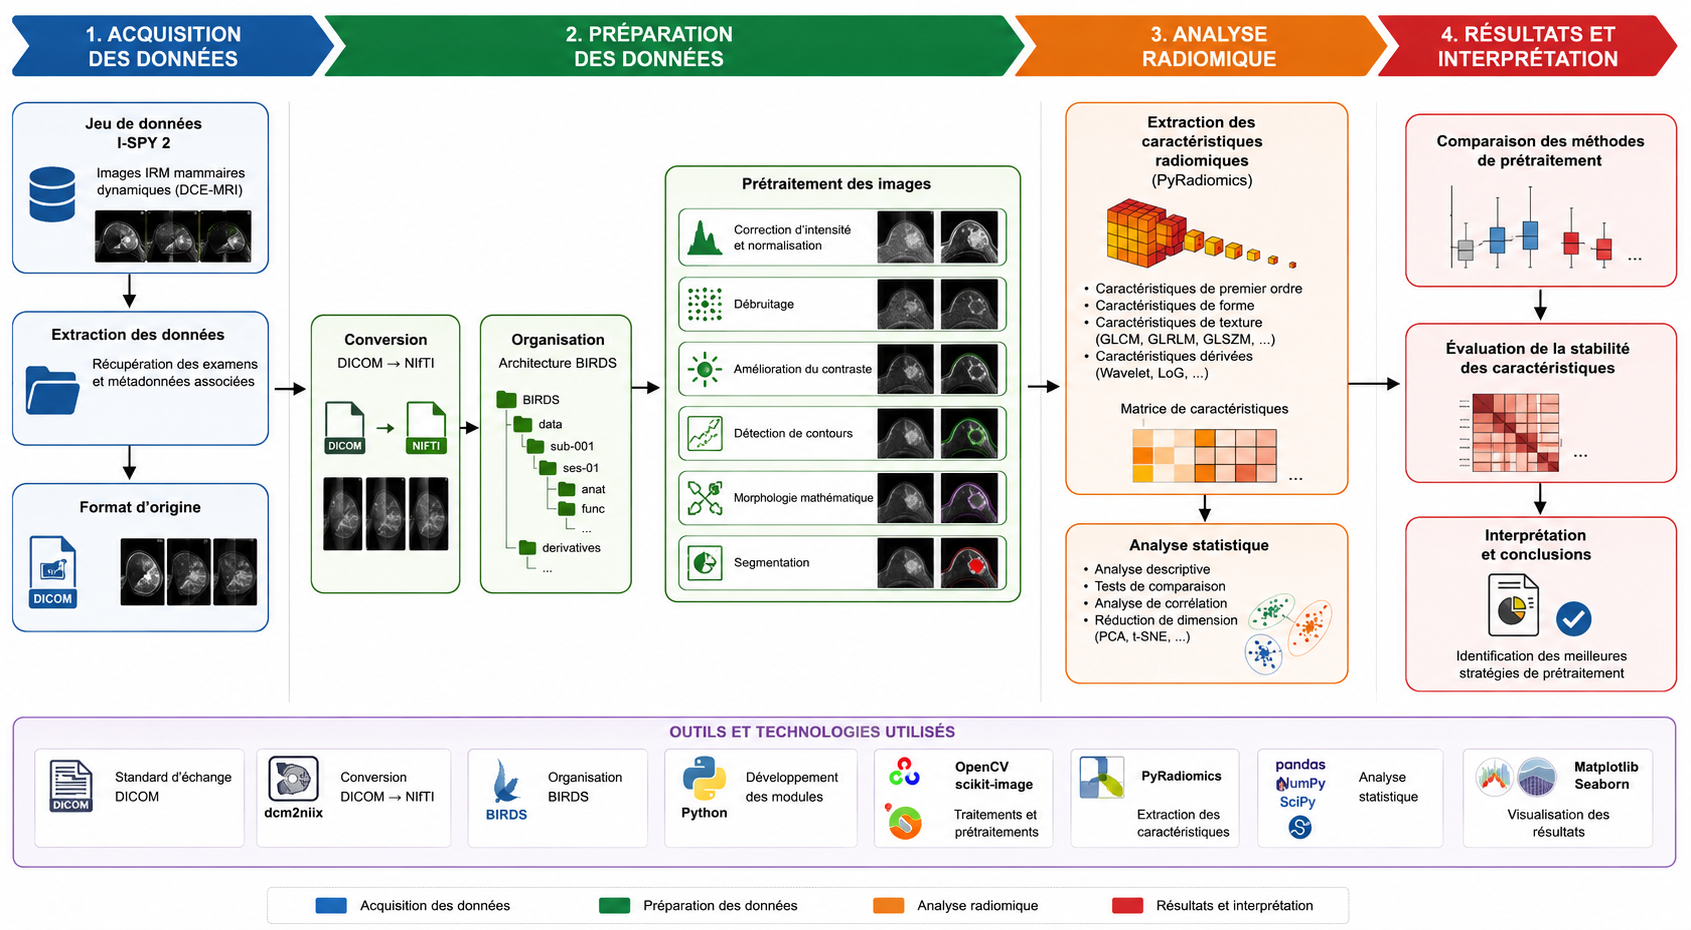
\includegraphics[width=0.85\textwidth]{Pipeline.png}
        \caption{Pipeline générale d'analyse des images médicales.}
        \label{fig:pipeline_generale}
    \end{figure}

    La Figure~\ref{fig:pipeline_generale} illustre le schéma général de la pipeline d'analyse d'images médicales. Ce schéma retrace de façon synthétique l'enchaînement des 7 étapes majeures : (1) l'acquisition et l'ingestion des données cliniques, (2) la conversion des séries DICOM vers le format NIfTI, (3) l'organisation standardisée des données selon le format BIDS, (4) l'application des traitements d'images au sein de la bibliothèque de prétraitement (correction N4, normalisation, débruitage, rehaussement de contraste), (5) la segmentation des régions d'intérêt (ROI), (6) l'extraction des caractéristiques radiomiques conformément aux directives de l'IBSI, et (7) l'analyse statistique comparative et la modélisation prédictive.

    \section{Problématique du sujet}
    
    Les études radiomiques font face à une forte variabilité liée aux appareils d'acquisition, aux protocoles, aux formats de stockage et aux méthodes de prétraitement. Ces variations artificielles risquent d'être confondues avec des variations biologiques réelles.
    
    \textbf{Formulation de la problématique :} \textit{Comment concevoir une pipeline modulaire, automatisée et reproductible appliquée aux images IRM du cancer du sein issues de la cohorte I-SPY 2, permettant d'évaluer objectivement l'influence des différentes méthodes de prétraitement sur la stabilité et la pertinence des caractéristiques radiomiques extraites ?}

    \section{Intérêt de l'étude}
    
    L'étude présente un triple intérêt :
    \begin{itemize}
        \item \textbf{Scientifique :} mesurer quantitativement l'impact des prétraitements sur la stabilité des biomarqueurs radiomiques conformément aux recommandations IBSI.
        \item \textbf{Technique :} développer une architecture logicielle Python modulaire, réutilisable et maintenable.
        \item \textbf{Applicatif :} fournir une infrastructure prête pour la préparation de données d'imagerie mammaire destinées à des modèles d'intelligence artificielle en oncologie.
    \end{itemize}

    \section{Objectifs du projet}
    
    \subsection{Objectif général}
    Développer une pipeline modulaire, automatisée et reproductible permettant la récupération, l'organisation, le prétraitement et l'analyse quantitative d'images IRM mammaires issues de la cohorte I-SPY 2.

    \subsection{Objectifs spécifiques}
    \begin{enumerate}
        \item \textbf{Extraction automatisée :} récupérer les séries DICOM et masques de la base I-SPY 2.
        \item \textbf{Conversion DICOM $\rightarrow$ NIfTI :} convertir les volumes avec préservation des métadonnées spatiales.
        \item \textbf{Organisation BIDS :} structurer les répertoires selon une architecture standardisée.
        \item \textbf{Bibliothèque de prétraitement :} implémenter des modules indépendants pour la correction N4, la normalisation, le débruitage, les filtres de contours et la segmentation.
        \item \textbf{Extraction radiomique (cadre prévus) :} définir les descripteurs IBSI/PyRadiomics à analyser.
        \item \textbf{Analyse statistique (cadre prévus) :} évaluer la stabilité des caractéristiques par métriques SNR, CNR, Dice et ICC.
    \end{enumerate}

    \section{Revue de la littérature}
    
    \subsection{Standards et formats de données}
    Les images médicales brutes sont fournies au format DICOM (NEMA). Pour les traitements scientifiques en Python, la conversion vers NIfTI (avec \texttt{dicom2nifti} ou \texttt{dcm2niix}) regroupe les coupes 3D en un fichier unique doté d'une matrice affine de transformation spatiale.
    
    L'organisation BIDS (\textit{Brain Imaging Data Structure}) normalise l'arborescence et le nommage des fichiers (\texttt{sub-XXX/ses-YYY/modalite/}), garantissant la reproductibilité et la traçabilité des transformations.

    \subsection{Méthodes de prétraitement des IRM}
    Le prétraitement regroupe :
    \begin{itemize}
        \item \textbf{Correction d'intensité :} l'algorithme N4ITK corrige l'inhomogénéité du champ radiofréquence ($B(x)$).
        \item \textbf{Normalisation :} Z-score ou normalisation robuste Min-Max par percentiles ($1\%-99\%$).
        \item \textbf{Débruitage :} filtres gaussien, anisotropique et Non-Local Means (NLM) adapté au bruit de Rician.
        \item \textbf{Rehaussement de contraste :} CLAHE, égalisation d'histogramme et correction Gamma.
        \item \textbf{Filtres de contours \& morphologie :} opérateurs Sobel, Canny, gradient morphologique et transformation Top-Hat.
        \item \textbf{Segmentation :} seuillage d'Otsu et post-traitement morphologique.
    \end{itemize}

    \subsection{Extraction radiomique et standardisation IBSI}
    PyRadiomics fournit des implémentations standardisées pour les caractéristiques de forme, de premier ordre et de matrices de texture (GLCM, GLRLM, GLSZM, GLDM, NGTDM). L'initiative IBSI définit les règles d'interpolation et de discrétisation indispensables à la reproductibilité inter-centre.

    \section{Solution proposée}
    
    La solution s'organise autour d'un flux modulaire complet :
    
    \begin{center}
    \small
    \begin{tcolorbox}[colframe=primaryblue,colback=lightgrey,halign=center]
    Jeu de données I-SPY 2 (TCIA)\\[2pt]
    $\downarrow$\\[2pt]
    Extraction automatisée des séries DICOM (\texttt{DATAUTILS})\\[2pt]
    $\downarrow$\\[2pt]
    Conversion DICOM $\rightarrow$ NIfTI (\texttt{dicom2nifti} / \texttt{NiBabel})\\[2pt]
    $\downarrow$\\[2pt]
    Organisation standardisée type BIDS (\texttt{dataset/derivatives/})\\[2pt]
    $\downarrow$\\[2pt]
    Bibliothèque modulaire de prétraitement (\texttt{PREPROCESSING}, \texttt{DENOISE}, \texttt{EDGES}, \texttt{MATHMORPHO}, \texttt{SEG})\\[2pt]
    $\downarrow$\\[2pt]
    Extraction des caractéristiques radiomiques \& Analyse statistique (Protocoles prévus)
    \end{tcolorbox}
    \end{center}

    \section*{Conclusion du chapitre}
    \addcontentsline{toc}{section}{Conclusion du chapitre}
    Ce chapitre a posé les bases théoriques de l'imagerie IRM mammaire, de la radiomique et des exigences de préparation des données. La revue de la littérature confirme la nécessité d'une pipeline modulaire et standardisée. Le chapitre suivant détaille la conception et l'implémentation de cette infrastructure.

    % =====================================================
    % CHAPITRE 2 : MATÉRIEL ET MÉTHODES
    % =====================================================
    \chapter{MATÉRIEL ET MÉTHODES}
    
    Ce chapitre présente la démarche méthodologique adoptée pour la conception et l'implémentation de la pipeline modulaire de traitement d'images IRM. Il décrit les jeux de données, l'infrastructure logicielle, la structure des modules Python développés et la formulation des méthodes de prétraitement.

    \section{Présentation générale}
    L'approche retenue repose sur une architecture logicielle découplée. Les données IRM de la cohorte I-SPY 2 sont ingérées, converties au format NIfTI, organisées sous forme BIDS puis soumises à une suite de modules de prétraitement et de segmentation.

    \section{Matériels}

    \subsection{Jeu de données I-SPY 2}
    Le sous-ensemble exploité dans les expérimentations comprend 5 patientes (\texttt{ISPY2-125130}, \texttt{ISPY2-227832}, \texttt{ISPY2-311455}, \texttt{ISPY2-313243}, \texttt{ISPY2-767081}), couvrant 4 sessions longitudinales (T0, T1, T2, T3), soit 20 sessions, 80 volumes DCE-MRI et 20 masques d'analyse.

    \begin{table}[H]
    \centering
    \caption{Caractéristiques du sous-ensemble du jeu de données I-SPY 2.}
    \label{tab:ispy2_summary}
    \begin{tabularx}{\textwidth}{>{\bfseries}p{4cm} X}
    \toprule
    Caractéristique & Description \\
    \midrule
    Source & The Cancer Imaging Archive (TCIA) \\
    Modalité & IRM dynamique avec contraste (DCE-MRI) \\
    Subjets inclus & 5 patientes (20 sessions longitudinales T0-T3) \\
    Format original & DICOM (19 160 fichiers) \\
    Format cible & NIfTI (\texttt{.nii.gz}, 100 fichiers produits) \\
    Orientation spatiale & RAS (Right-Anterior-Superior) \\
    \bottomrule
    \end{tabularx}
    \end{table}

    \begin{figure}[H]
    \centering
    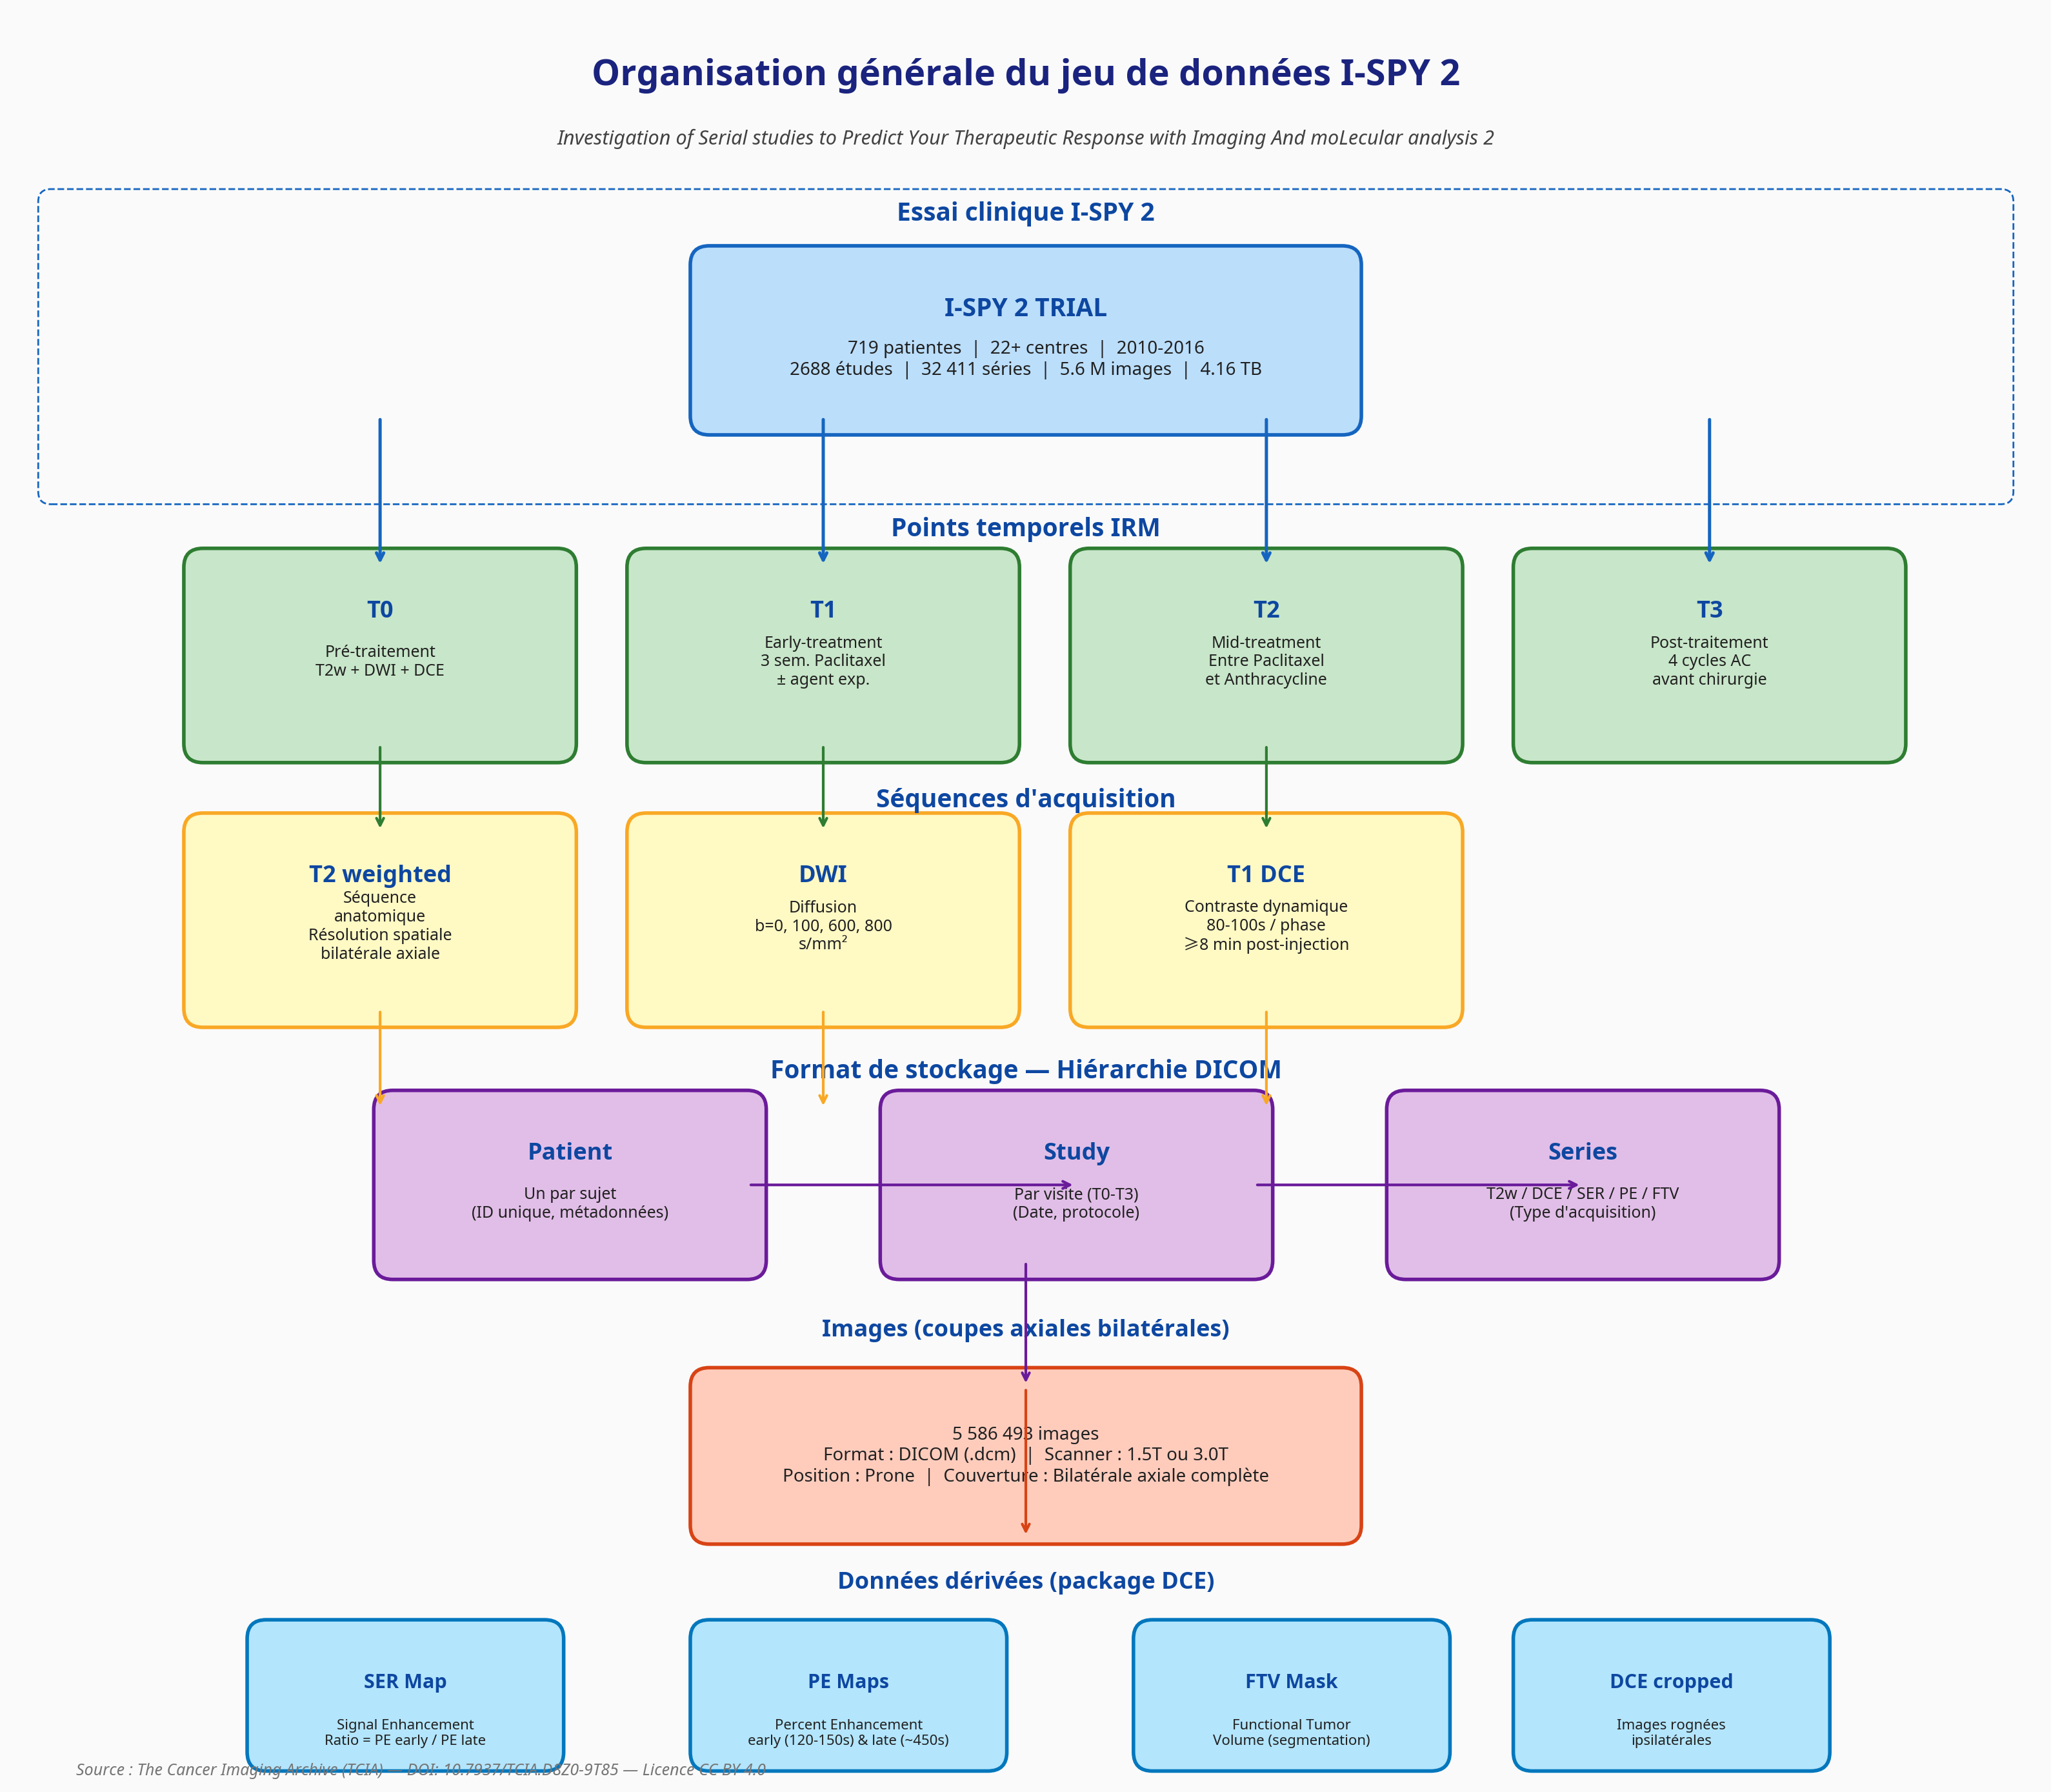
\includegraphics[width=0.85\textwidth]{ispy2_dataset.png}
    \caption{Illustration du jeu de données I-SPY 2 et des acquisitions IRM utilisées dans cette étude.}
    \label{fig:ispy2_dataset_ch2}
    \end{figure}

    La Figure~\ref{fig:ispy2_dataset_ch2} détaille la structure modale et temporelle de la cohorte I-SPY 2 exploitée. Elle présente l'organisation des examens d'imagerie par résonance magnétique dynamique avec injection de produit de contraste (DCE-MRI) acquis à 4 jalons temporels du traitement néoadjuvant ($T_0, T_1, T_2, T_3$). Chaque examen comprend les phases d'imagerie anatomique ainsi que les masques de segmentation tumorale de référence validés par les radiologues.

    \subsection{Organisation des données selon le standard BIDS}
    Les fichiers convertis sont organisés selon une structure dérivée de BIDS :
    \begin{figure}[H]
    \centering
    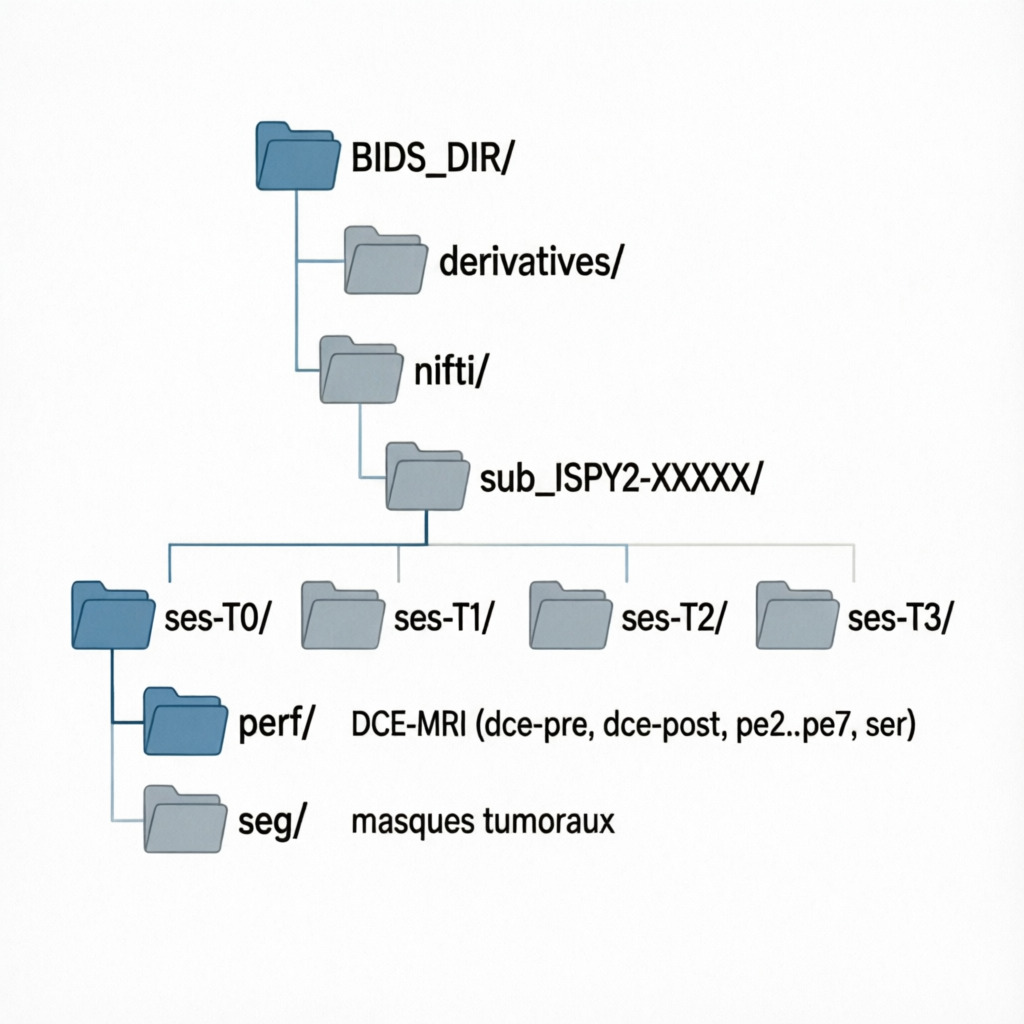
\includegraphics[width=0.85\textwidth]{bids_structure.png}
    \caption{Organisation des données selon une structure inspirée du standard BIDS.}
    \label{fig:bids_structure_ch2}
    \end{figure}

    La Figure~\ref{fig:bids_structure_ch2} présente l'arborescence normalisée adaptée aux spécificités de l'imagerie mammaire. La structure sépare les données sources originales des données dérivées (\texttt{derivatives/}). Chaque sujet est répertorié dans un dossier spécifique (\texttt{sub-ISPY2-xxxxx/}) découpé par session (\texttt{ses-Tx/}), classant d'un côté les volumes d'imagerie DCE (\texttt{perf/}) et de l'autre les masques de référence (\texttt{seg/}), garantissant ainsi la traçabilité absolue de chaque traitement.

    \subsection{Environnement de développement \& matériel}
    Le développement est réalisé en Python 3.13 sous Ubuntu Linux. L'environnement repose sur les bibliothèques scientifiques présentées au Tableau~\ref{tab:logiciels}.

    \begin{table}[H]
    \centering
    \caption{Bibliothèques logicielles principales.}
    \label{tab:logiciels}
    \begin{tabularx}{\textwidth}{>{\bfseries}p{3.5cm} >{\bfseries}p{3cm} X}
    \toprule
    Domaine & Bibliothèque & Rôle \\
    \midrule
    DICOM \& NIfTI & \texttt{pydicom}, \texttt{dicom2nifti}, \texttt{nibabel} & Lecture, conversion et manipulation des métadonnées. \\
    Traitement d'image & \texttt{SimpleITK}, \texttt{scikit-image}, \texttt{OpenCV} & Correction N4, filtrage, morphologie et segmentation. \\
    Calculs & \texttt{NumPy}, \texttt{SciPy} & Opérations matricielles et traitement du signal. \\
    Visualisation & \texttt{Matplotlib}, \texttt{Seaborn} & Génération des figures 2D, multiplanaires 3D et graphiques. \\
    \bottomrule
    \end{tabularx}
    \end{table}

    \section{Conception de la pipeline}

    \subsection{Architecture générale \& Diagramme fonctionnel}
    La Figure~\ref{fig:diagramme_pipeline} illustre le flux fonctionnel de traitement d'un volume IRM.

    \begin{figure}[H]
        \centering
        \includegraphics[width=0.62\textwidth]{diagrams/pipeline_diagram.png}
        \caption{Diagramme fonctionnel du traitement et de l'évaluation d'une IRM DCE.}
        \label{fig:diagramme_pipeline}
    \end{figure}

    La Figure~\ref{fig:diagramme_pipeline} détaille le flux d'exécution fonctionnel appliqué à un volume IRM DCE. Le workflow débute par l'importation du volume NIfTI d'entrée, suivi de la correction de champ de biais N4 et de la normalisation d'intensité. Le volume prétraité alimente ensuite les algorithmes de réduction de bruit (NLM Rician et diffusion anisotropique) ainsi que les opérateurs morphologiques. Deux voies de segmentation sont intégrées : la méthode exploratoire par seuillage automatique d'Otsu et la branche utilisant le masque de référence. La comparaison spatiale des masques permet enfin le calcul automatique des métriques de performance (Dice, IoU, sensibilité, spécificité, Hausdorff 95).

    \subsection{Architecture logicielle en packages Python}
    L'implémentation est découpée en packages modulaires sous le répertoire \texttt{src/} :
    \begin{itemize}
        \item \textbf{DATAUTILS :} gestion de l'ingestion TCIA, de la conversion DICOM $\rightarrow$ NIfTI et de l'arborescence BIDS.
        \item \textbf{MEDIO :} encapsulation objet du volume 3D, de l'affine et du masque via \texttt{MedicalImage3D}.
        \item \textbf{PREPROCESSING :} algorithmes de correction N4, normalisation Z-score/Min-Max et CLAHE.
        \item \textbf{DENOISE :} filtres Gaussien, Diffusion Anisotrope et NLM Rician.
        \item \textbf{EDGES \& MATHMORPHO :} opérateurs Sobel, Canny, gradient morphologique et Top-Hat.
        \item \textbf{SEG \& SEGUTILS :} stratégies de segmentation (Otsu, K-Means, FCM) et métriques d'évaluation (Dice, IoU, Hausdorff 95).
    \end{itemize}

    \begin{figure}[H]
        \centering
        \includegraphics[width=0.68\textwidth]{diagrams/package_diagram.png}
        \caption{Architecture des packages Python et de leurs dépendances principales.}
        \label{fig:diagramme_packages}
    \end{figure}

    La Figure~\ref{fig:diagramme_packages} illustre l'organisation modulaire des packages Python composant la solution sous \texttt{src/}. Chaque package possède une responsabilité distincte : \texttt{datautils} s'occupe de l'acquisition et de la conversion BIDS, \texttt{medio} fournit les structures mémoire d'images 3D, \texttt{preprocessing} et \texttt{denoise} gèrent la correction d'intensité et le filtrage, \texttt{edges} et \texttt{mathmorpho} extraient la géométrie locale et la morphologie, tandis que \texttt{seg} et \texttt{segutils} regroupent les algorithmes et métriques de segmentation.

    \begin{figure}[H]
        \centering
        \includegraphics[width=0.68\textwidth]{diagrams/class_diagram_core.png}
        \caption{Dépendances entre les modules centraux de traitement des images.}
        \label{fig:diagramme_core}
    \end{figure}

    La Figure~\ref{fig:diagramme_core} présente les dépendances entre les classes centrales du projet. La classe pivot \texttt{MedicalImage3D} encapsule sous forme d'un objet unique le tableau de voxels tridimensionnel (\texttt{numpy.ndarray}), la matrice de transformation affine 4x4, l'en-tête de métadonnées NIfTI et le masque de région d'intérêt. Cette encapsulation unifiée permet de transmettre l'image et sa géométrie à travers tous les modules de traitement de manière fluide et sécurisée.

    \section{Modules de la pipeline}

    \subsection{Extraction, Conversion et BIDS}
    Le module d'ingestion automatise le téléchargement des séries DCE et leur conversion. Les métadonnées de positionnement spatial (affine matrix, voxel spacing) sont transmises directement à la classe \texttt{MedicalImage3D}.

    \begin{figure}[H]
        \centering
        \includegraphics[width=0.88\textwidth]{diagrams/sequence_ispy2.png}
        \caption{Séquence d'extraction, de conversion et de stockage des données I-SPY 2.}
        \label{fig:sequence_ispy2}
    \end{figure}

    La Figure~\ref{fig:sequence_ispy2} détaille le diagramme de séquence chronologique régissant le téléchargement et la conversion des séries médicales. L'utilisateur déclenche l'exécution via \texttt{DataExtractor}, qui interroge l'API TCIA/NBIA, télécharge les séries DICOM et les enregistre localement. Le module \texttt{DicomConverter} convertit ensuite les fichiers DICOM en un volume NIfTI compressé. Enfin, \texttt{NiBabel} valide l'intégrité du volume et de l'affine RAS avant la création de l'objet \texttt{MedicalImage3D}.

    \subsection{Bibliothèque de prétraitement et Diagrammes de classes}
    Les Figures~\ref{fig:diagramme_preparation}, \ref{fig:diagramme_morphologie} et \ref{fig:diagramme_segmentation} présentent les diagrammes UML des modules de prétraitement, morphologie et segmentation.

    \begin{figure}[H]
        \centering
        \includegraphics[width=0.72\textwidth]{diagrams/class_diagram_preparation.png}
        \caption{Classes et méthodes dédiées à la préparation des images.}
        \label{fig:diagramme_preparation}
    \end{figure}

    La Figure~\ref{fig:diagramme_preparation} expose les classes de prétraitement et de correction d'intensité (\texttt{N4BiasFieldCorrection}, \texttt{RobustMinMaxNormalizer}, \texttt{ZScoreNormalizer}, \texttt{CLAHEEnhancer}). Ces classes héritent toutes de l'interface commune \texttt{BaseImageTransform}, implémentant le design pattern \textit{Strategy}. Cette conception permet de permuter facilement différentes techniques de correction et de normalisation sans modifier le code client de la pipeline.

    \begin{figure}[H]
        \centering
        \includegraphics[width=0.62\textwidth]{diagrams/class_diagram_morphology_analysis.png}
        \caption{Classes dédiées aux opérations morphologiques et à l'analyse de forme.}
        \label{fig:diagramme_morphologie}
    \end{figure}

    La Figure~\ref{fig:diagramme_morphologie} présente le diagramme de classes dédié aux opérations de morphologie mathématique 3D et d'analyse de forme. La classe \texttt{MorphologicalGradient} extrait les contours par différence entre dilatation et érosion 3D, \texttt{WhiteTopHat} isole les éléments clairs de petite taille par rapport au fond, et \texttt{MorphoCleaner} applique des ouvertures et fermetures volumiques pour supprimer le bruit de fond et lisser les masques.

    \begin{figure}[H]
        \centering
        \includegraphics[width=0.68\textwidth]{diagrams/class_diagram_segmentation_evaluation.png}
        \caption{Stratégies de segmentation et outils d'évaluation des masques.}
        \label{fig:diagramme_segmentation}
    \end{figure}

    La Figure~\ref{fig:diagramme_segmentation} illustre la hiérarchie des stratégies de segmentation et de leurs modules d'évaluation. Les algorithmes (\texttt{OtsuSegmenter}, \texttt{KMeansSegmenter}, \texttt{FCMSegmenter}) implémentent l'interface \texttt{SegmentationStrategy}. La classe \texttt{SegmentationEvaluator} pilote le calcul des métriques de concordance spatiale via des sous-classes dédiées : \texttt{DiceMetric}, \texttt{IoUMetric}, \texttt{Hausdorff95Metric} et \texttt{VolumeSimilarityMetric}.

    \section{Méthodes de prétraitement}
    La bibliothèque regroupe l'ensemble des méthodes dont la formulation théorique est résumée ci-dessous :
    
    \begin{itemize}
        \item \textbf{Correction N4 :} modèle multiplicatif $I(x) = J(x) \cdot B(x) + e(x)$, où $B(x)$ est estimé par B-splines lisses dans le domaine logarithmique.
        \item \textbf{Normalisation robuste :} $I_{norm}(x) = \frac{I(x) - P_1}{P_{99} - P_1}$, ramenant les intensités dans $[0, 1]$.
        \item \textbf{Débruitage NLM Rician :} étudie les patchs d'intensité avec correction du biais de bruit rician $\sigma^2$.
        \item \textbf{Opérateurs de contours :} gradient Sobel $G = \sqrt{G_x^2 + G_y^2 + G_z^2}$ et détection hystérésis de Canny.
        \item \textbf{Seuillage d'Otsu :} maximisation de la variance inter-classe $\sigma_B^2(t) = w_0(t)w_1(t)[\mu_0(t) - \mu_1(t)]^2$.
    \end{itemize}

    \section{Protocoles d'extraction radiomique et d'analyse statistique}
    Le protocole d'analyse prévu définit l'extraction via PyRadiomics (conforme IBSI) des caractéristiques 3D (First Order, Shape, GLCM, GLRLM, GLSZM) ainsi que l'évaluation de leur stabilité inter-traitement par le coefficient de corrélation intraclasse (ICC) et les tests statistiques appariés.

    \section*{Conclusion du chapitre}
    \addcontentsline{toc}{section}{Conclusion du chapitre}
    Ce chapitre a détaillé la conception modulaire, l'architecture logicielle des packages Python et la formulation des méthodes de prétraitement. Le chapitre suivant présente les résultats expérimentaux et leur discussion.

    % =====================================================
    % CHAPITRE 3 : RÉSULTATS ET DISCUSSION
    % =====================================================
    \chapter{Résultats et discussion}
\label{chap:resultats_discussion}

\section{Présentation des résultats}
\label{sec:presentation_resultats}

Ce chapitre présente les résultats obtenus après l'exécution de la pipeline de traitement sur le sous-ensemble disponible de la collection I-SPY 2. L'inventaire des données porte sur cinq patientes et quatre sessions longitudinales par patiente, de T0 à T3. En revanche, l'exécution complète des modules de prétraitement et de génération des figures a été réalisée sur un exemple reproductible : la patiente \texttt{ISPY2-125130}, session \texttt{T0}, série \texttt{dce-post-1}. Cette distinction permet de ne pas confondre les données disponibles avec les données effectivement traitées dans l'expérience présentée.

Les résultats sont présentés selon les principales étapes de la pipeline : extraction des données DICOM, conversion au format NIfTI, organisation des fichiers, prétraitement des volumes, segmentation et préparation de l'analyse quantitative. Les résultats directement vérifiables dans le répertoire expérimental sont distingués des résultats qui nécessitent encore l'exécution d'un module radiomique et d'une analyse statistique complète.

\section{Résultats des différents modules de la pipeline}
\label{sec:resultats_modules}

\subsection{Résultats de l'extraction des données}
\label{subsec:resultats_extraction}

L'extraction a permis de récupérer les données de cinq patientes : \texttt{ISPY2-125130}, \texttt{ISPY2-227832}, \texttt{ISPY2-311455}, \texttt{ISPY2-313243} et \texttt{ISPY2-767081}. Les quatre sessions attendues ont été retrouvées pour chacune d'elles, soit un total de 20 sessions.

Les données DICOM sont conservées dans une arborescence organisée par patiente et par session. Le répertoire contient 19\,160 fichiers DICOM. Les séries téléchargées correspondent aux acquisitions DCE originales et aux séries d'analyse contenant les masques. Après extraction des phases temporelles, chaque session dispose des volumes \texttt{dce-pre}, \texttt{dce-post-1}, \texttt{dce-post-2}, \texttt{dce-post-3} ainsi que d'un masque.

Un contrôle des métadonnées a été réalisé sur les séries disponibles. Les champs nécessaires à la conversion et au classement --- notamment \texttt{PatientID}, \texttt{StudyInstanceUID}, \texttt{SeriesInstanceUID}, \texttt{SeriesDescription}, \texttt{Rows}, \texttt{Columns} et \texttt{InstanceNumber} --- sont présents dans les fichiers contrôlés. Les 140 répertoires de séries examinés présentent un identifiant \texttt{SeriesInstanceUID} unique, ce qui indique que les séries retenues ne sont pas mélangées entre plusieurs acquisitions.

\subsection{\texorpdfstring{Résultats de la conversion DICOM $\rightarrow$ NIfTI}{Résultats de la conversion DICOM vers NIfTI}}
\label{subsec:resultats_conversion}

La conversion a produit 100 fichiers NIfTI de référence : 80 volumes d'imagerie, correspondant à quatre phases DCE pour chacune des 20 sessions, et 20 masques de segmentation. Les volumes sont enregistrés au format compressé \texttt{.nii.gz}.

Les contrôles effectués après conversion montrent que les 100 fichiers sont lisibles, non vides et contiennent uniquement des valeurs finies. Ils sont tous orientés selon le repère RAS. Pour chacune des 20 sessions, la dimension du masque correspond à celle des volumes DCE associés, ce qui permet leur utilisation conjointe pour les traitements ultérieurs.

Les dimensions observées varient selon les acquisitions. Les principales tailles sont \texttt{(256, 256, 64)}, \texttt{(256, 256, 80)}, \texttt{(256, 256, 134)} et \texttt{(312, 312, 80)}. Cette variabilité montre que les acquisitions n'ont pas toutes été réalisées avec les mêmes paramètres spatiaux. Les espacements de voxels varient également, avec des valeurs comprises approximativement entre 0,586 et 0,962 mm dans le plan et entre 1,2 et 2,5 mm selon l'axe des coupes.

Les volumes d'imagerie sont stockés en \texttt{uint16}, tandis que les masques sont stockés en \texttt{uint8}. Le masque n'est pas strictly binaire : plusieurs étiquettes sont présentes, notamment les valeurs 1, 2, 17, 32, 33, 34 et 49. Dans les traitements utilisant un masque binaire, la présence d'un voxel dans le masque est considérée par la condition \texttt{masque > 0}. Cette précision est importante pour l'interprétation des résultats de segmentation et de radiomique.

\begin{figure}[H]
    \centering
    \includegraphics[width=0.82\textwidth]{../results/sub-ISPY2-125130/ses-T0/figures/2d/01_original.png}
    \caption{Coupe axiale du volume DCE sélectionné après conversion au format NIfTI ($X=108$, $Y=87$, $Z=27$).}
    \label{fig:resultat_original}
\end{figure}

La coupe originale présente une anatomie mammaire clairement visible et une zone de signal élevé dans la région centrale de la lésion. Cette image sert de référence visuelle pour toutes les comparaisons suivantes. Elle est affichée avec une fenêtre d'intensité robuste ; les niveaux de gris observés ne doivent donc pas être interprétés comme une mesure absolue indépendante de la méthode d'affichage.

\subsection{Résultats de l'organisation des données selon BIDS}
\label{subsec:resultats_bids}

L'organisation finale suit une structure de type BIDS dérivée :

\begin{lstlisting}[basicstyle=\small\ttfamily]
ISPY2_dataset/
|-- derivatives/
|   |-- nifti/
|       |-- sub-ISPY2-xxxxx/
|           |-- ses-Tx/
|               |-- perf/
|               |   |-- *_dce-pre.nii.gz
|               |   |-- *_dce-post-1.nii.gz
|               |   |-- *_dce-post-2.nii.gz
|               |   +-- *_dce-post-3.nii.gz
|               +-- seg/
|                   +-- *_mask.nii.gz
\end{lstlisting}

Les cinq dossiers sujets contiennent chacun quatre dossiers de session. Les répertoires \texttt{perf} contiennent 80 volumes DCE au total et les répertoires \texttt{seg} contiennent 20 masques. La structure est donc complète pour les quatre temps étudiés. Un fichier supplémentaire, obtenu après l'exécution du module de débruitage, est présent pour la session T0 de la patiente \texttt{ISPY2-125130} ; il s'agit d'un dérivé de traitement et non d'un volume issu de la conversion initiale.

La validation de l'arborescence montre que chaque session possède les deux types de données attendus et que les noms de fichiers permettent d'identifier la patiente, la session et la phase temporelle. Cette organisation facilite l'automatisation des traitements et la traçabilité des résultats.

\subsection{Résultats des méthodes de prétraitement}
\label{subsec:resultats_pretraitement}

Les méthodes implémentées dans la pipeline concernent la correction d'intensité, la normalisation, l'amélioration du contraste, le débruitage, la détection de contours, la morphologie mathématique et la segmentation.

La correction de champ de biais vise à réduire les variations lentes d'intensité qui ne correspondent pas à une différence anatomique réelle. La normalisation robuste par percentiles, utilisée avec les percentiles 1 et 99, ramène les intensités utiles dans un intervalle comparable tout en limitant l'influence des valeurs extrêmes. Ces traitements modifient l'échelle des intensités ; ils doivent donc être appliqués de manière identique à l'ensemble des sujets et des sessions lorsqu'une comparaison quantitative est réalisée.

Le débruitage est réalisé à l'aide d'un filtre non local adapté au bruit de type Rician, suivi d'un filtrage anisotropique. L'observation qualitative attendue est une diminution des fluctuations locales dans les régions homogènes, avec une préservation relative des transitions anatomiques. Pour l'exemple disponible, le débruitage du volume \texttt{sub-ISPY2-125130\_}\allowbreak\texttt{ses-T0\_}\allowbreak\texttt{dce-post-1} conserve une corrélation élevée avec l'image originale ($r = 0{,}998$ dans le masque utilisé), tandis que l'écart absolu moyen entre les deux volumes est d'environ $4{,}93$ unités d'intensité. Cela indique une modification modérée des intensités, principalement destinée à atténuer les variations locales.

La morphologie mathématique est utilisée pour produire un gradient morphologique, améliorer certaines structures par transformation top-hat et nettoyer les masques. Ces opérations facilitent l'analyse des contours et la suppression de petites composantes ou de petits trous. Les détecteurs de Canny et de Sobel fournissent ensuite deux représentations complémentaires des transitions d'intensité : Canny produit des contours plus sélectifs, tandis que Sobel fournit une réponse basée sur le gradient local.

La segmentation par seuillage d'Otsu constitue une première méthode automatique. Le post-traitement comprend la suppression des petites composantes et le remplissage des trous. Cette segmentation doit être interprétée comme une étape exploratoire : son efficacité dépend du contraste entre la région d'intérêt et les tissus environnants et ne peut être jugée définitivement qu'au moyen d'une comparaison avec un masque de référence.

\begin{figure}[H]
    \centering
    \includegraphics[width=0.47\textwidth]{../results/sub-ISPY2-125130/ses-T0/figures/2d/01_original.png}\hfill
    \includegraphics[width=0.47\textwidth]{../results/sub-ISPY2-125130/ses-T0/figures/2d/02_bias_corrected.png}\\[0.3cm]
    \includegraphics[width=0.47\textwidth]{../results/sub-ISPY2-125130/ses-T0/figures/2d/03_robust_minmax.png}\hfill
    \includegraphics[width=0.47\textwidth]{../results/sub-ISPY2-125130/ses-T0/figures/2d/04_denoised.png}
    \caption{Comparaison 2D : image originale, correction de biais N4, normalisation robuste min-max et volume débruité.}
    \label{fig:resultats_pretraitement}
\end{figure}

La correction de biais modifie principalement les variations lentes de l'intensité dans le volume, sans déplacer les structures anatomiques. La normalisation robuste améliore la comparabilité de l'échelle d'affichage en limitant l'effet des valeurs extrêmes. Le débruitage produit une image plus lisse, notamment dans les régions relativement homogènes, tout en conservant les contours principaux. Dans l'exemple traité, la corrélation avec l'image originale est de $r=0{,}998$ et l'écart absolu moyen est d'environ $4{,}93$ unités, ce qui indique une modification modérée plutôt qu'une transformation structurelle du volume.

\begin{figure}[H]
    \centering
    \includegraphics[width=0.47\textwidth]{../results/sub-ISPY2-125130/ses-T0/figures/2d/05_reference_mask.png}\hfill
    \includegraphics[width=0.47\textwidth]{../results/sub-ISPY2-125130/ses-T0/figures/2d/06_cleaned_mask.png}\\[0.3cm]
    \includegraphics[width=0.47\textwidth]{../results/sub-ISPY2-125130/ses-T0/figures/2d/09_otsu.png}\hfill
    \includegraphics[width=0.47\textwidth]{../results/sub-ISPY2-125130/ses-T0/figures/2d/10_otsu_cleaned.png}
    \caption{Masque de référence, masque nettoyé et résultats de la segmentation par seuillage d'Otsu (brut et nettoyé).}
    \label{fig:resultats_segmentation}
\end{figure}

Le masque de référence contient plusieurs étiquettes et ne correspond donc pas à une simple image en niveaux de gris. Après binarisation et nettoyage, le masque devient plus lisible pour les opérations morphologiques et l'évaluation. La segmentation Otsu détecte cependant de nombreuses régions de forte intensité qui ne correspondent pas toutes à la région d'intérêt. Cette sur-segmentation est visible dans la comparaison avec le masque de référence et explique les faibles valeurs obtenues pour le Dice ($0{,}1802$), l'IoU ($0{,}0990$) et la sensibilité ($0{,}0994$). La précision élevée ($0{,}9607$) doit être interprétée avec prudence : elle ne compense pas la faible détection de la région cible.

\begin{figure}[H]
    \centering
    \includegraphics[width=0.85\textwidth]{../results/sub-ISPY2-125130/ses-T0/figures/pipeline_overview.png}
    \caption{Vue d'ensemble synthétique de l'exécution du workflow sur le volume IRM du sujet sub-ISPY2-125130.}
    \label{fig:pipeline_overview}
\end{figure}

\begin{figure}[H]
    \centering
    \includegraphics[width=0.47\textwidth]{../results/sub-ISPY2-125130/ses-T0/figures/2d/07_morphological_gradient.png}\hfill
    \includegraphics[width=0.47\textwidth]{../results/sub-ISPY2-125130/ses-T0/figures/2d/08_white_tophat.png}\\[0.3cm]
    \includegraphics[width=0.47\textwidth]{../results/sub-ISPY2-125130/ses-T0/figures/2d/11_canny.png}\hfill
    \includegraphics[width=0.47\textwidth]{../results/sub-ISPY2-125130/ses-T0/figures/2d/12_sobel.png}
    \caption{Coupes axiales 2D des traitements morphologiques (gradient et top-hat) et des détecteurs de contours (Canny et Sobel).}
    \label{fig:resultats_2d_morpho_edges}
\end{figure}

\subsection{Galerie des visualisations multiplanaires tridimensionnelles}
\label{subsec:galerie_multiplanaire}

Afin d'évaluer la cohérence spatiale 3D des traitements appliqués sur l'ensemble du volume IRM, des représentations multiplanaires combinant les coupes axiales ($X=108$), coronales ($Y=87$), sagittales ($Z=27$) ainsi qu'un rendu tridimensionnel volumique ont été générées pour chaque étape du workflow.

La Figure~\ref{fig:multiplanar_pretraitement} présente les vues multiplanaires des différentes étapes de préparation de l'image.

\begin{figure}[H]
    \centering
    \includegraphics[width=0.47\textwidth]{../results/sub-ISPY2-125130/ses-T0/figures/multiplanar/01_original.png}\hfill
    \includegraphics[width=0.47\textwidth]{../results/sub-ISPY2-125130/ses-T0/figures/multiplanar/02_bias_corrected.png}\\[0.3cm]
    \includegraphics[width=0.47\textwidth]{../results/sub-ISPY2-125130/ses-T0/figures/multiplanar/03_robust_minmax.png}\hfill
    \includegraphics[width=0.47\textwidth]{../results/sub-ISPY2-125130/ses-T0/figures/multiplanar/04_denoised.png}
    \caption{Vues multiplanaires (axiale, coronale, sagittale et rendu 3D) des étapes de prétraitement : volume original, correction de champ de biais, normalisation robuste et volume débruité.}
    \label{fig:multiplanar_pretraitement}
\end{figure}

La Figure~\ref{fig:multiplanar_segmentation} illustre les représentations multiplanaires des masques de référence et des résultats de segmentation.

\begin{figure}[H]
    \centering
    \includegraphics[width=0.47\textwidth]{../results/sub-ISPY2-125130/ses-T0/figures/multiplanar/05_reference_mask.png}\hfill
    \includegraphics[width=0.47\textwidth]{../results/sub-ISPY2-125130/ses-T0/figures/multiplanar/06_cleaned_mask.png}\\[0.3cm]
    \includegraphics[width=0.47\textwidth]{../results/sub-ISPY2-125130/ses-T0/figures/multiplanar/09_otsu.png}\hfill
    \includegraphics[width=0.47\textwidth]{../results/sub-ISPY2-125130/ses-T0/figures/multiplanar/10_otsu_cleaned.png}
    \caption{Vues multiplanaires des masques et de la segmentation : masque de référence, masque nettoyé, segmentation par seuillage d'Otsu et masque Otsu nettoyé.}
    \label{fig:multiplanar_segmentation}
\end{figure}

Enfin, la Figure~\ref{fig:multiplanar_morpho_edges} présente les vues multiplanaires obtenues pour les filtres morphologiques et les opérateurs de détection de contours.

\begin{figure}[H]
    \centering
    \includegraphics[width=0.47\textwidth]{../results/sub-ISPY2-125130/ses-T0/figures/multiplanar/07_morphological_gradient.png}\hfill
    \includegraphics[width=0.47\textwidth]{../results/sub-ISPY2-125130/ses-T0/figures/multiplanar/08_white_tophat.png}\\[0.3cm]
    \includegraphics[width=0.47\textwidth]{../results/sub-ISPY2-125130/ses-T0/figures/multiplanar/11_canny.png}\hfill
    \includegraphics[width=0.47\textwidth]{../results/sub-ISPY2-125130/ses-T0/figures/multiplanar/12_sobel.png}
    \caption{Vues multiplanaires des filtres morphologiques et des détections de contours : gradient morphologique, transformation top-hat, détecteur de Canny et filtre de Sobel.}
    \label{fig:multiplanar_morpho_edges}
\end{figure}

Les vues multiplanaires confirment que l'ensemble des traitements est appliqué de manière tridimensionnelle et volumétrique cohérente sur l'ensemble des plans d'imagerie IRM.

Les métriques calculées pour la segmentation Otsu nettoyée, comparée au masque de référence, sont présentées dans le tableau suivant :

\begin{table}[H]
\centering
\caption{Évaluation de la segmentation Otsu sur l'exemple traité.}
\label{tab:metriques_otsu}
\begin{tabular}{lr}
\toprule
Métrique & Valeur \\
\midrule
Dice & 0,1802 \\
IoU & 0,0990 \\
Sensibilité & 0,0994 \\
Spécificité & 0,0001 \\
Précision & 0,9607 \\
Hausdorff 95 & 52,1282 \\
Similarité de volume & 0,1035 \\
\bottomrule
\end{tabular}
\end{table}

Ces valeurs montrent que la segmentation Otsu constitue uniquement une approche exploratoire dans cette expérience. Le faible coefficient de Dice et la faible sensibilité indiquent une correspondance limitée avec le masque de référence ; la précision élevée ne suffit donc pas à conclure à une bonne segmentation.

\subsection{Résultats de l'extraction radiomique}
\label{subsec:resultats_radiomique}

Dans l'état actuel du projet, aucun fichier CSV de caractéristiques radiomiques n'est présent dans l'arborescence. Le nombre total de caractéristiques extraites, leur répartition par famille et les statistiques descriptives ne peuvent donc pas être rapportés comme des résultats expérimentaux définitifs.

La prochaine étape devra appliquer une configuration radiomique fixée aux mêmes couples image--masque. Le tableau de résultats devra au minimum contenir l'identifiant de la patiente, la session, la phase DCE, la méthode de prétraitement, le nom de la caractéristique et sa valeur. Les familles attendues sont les suivantes : First Order, Shape, GLCM, GLRLM, GLSZM, GLDM et NGTDM.

Un exemple de ligne de résultats pourra contenir les champs suivants : sujet, session, phase, prétraitement, caractéristique et valeur. Par exemple :

\begin{lstlisting}[basicstyle=\small\ttfamily]
ISPY2-xxxxx | T0 | dce-post-1 | original   | FirstOrder_Mean | a completer
ISPY2-xxxxx | T0 | dce-post-1 | debruitage | FirstOrder_Mean | a completer
\end{lstlisting}

Les paramètres de discrétisation, le nombre de niveaux de gris, le type de masque et la configuration spatiale devront être conservés dans la méthodologie afin de rendre les caractéristiques reproductibles.

\section{Analyse statistique}
\label{sec:analyse_statistique}

\subsection{Comparaison des méthodes de prétraitement}
\label{subsec:comparaison_pretraitement}

La comparaison statistique devra être réalisée à partir des mêmes sujets, sessions, phases et masques afin d'éviter que les différences observées ne soient dues à une composition différente des groupes. Pour chaque caractéristique, il conviendra d'examiner sa moyenne, son écart-type, sa médiane, son intervalle interquartile et son coefficient de variation.

La stabilité pourra être étudiée en comparant les valeurs obtenues avant et après prétraitement. La reproductibilité pourra être résumée par un coefficient de corrélation intraclasse ou par une mesure de concordance adaptée au plan expérimental. Les tests statistiques devront tenir compte du caractère apparié des observations lorsque plusieurs méthodes sont appliquées au même volume.

Les valeurs numériques de ces comparaisons restent à compléter, car aucun tableau de caractéristiques radiomiques ni fichier de sortie statistique n'est actuellement disponible dans le projet.

\subsection{Visualisation des résultats}
\label{subsec:visualisation_resultats}

Les visualisations recommandées sont les suivantes :

\begin{itemize}
    \item des \textit{boxplots} pour comparer les distributions d'une caractéristique entre méthodes ;
    \item des histogrammes pour visualiser les modifications d'intensité ;
    \item des \textit{heatmaps} pour représenter les valeurs standardisées des caractéristiques ;
    \item des matrices de corrélation pour étudier la redondance entre caractéristiques ;
    \item des graphiques comparatifs pour classer les méthodes selon la stabilité ou la reproductibilité.
\end{itemize}

Chaque figure devra préciser la phase DCE, la session, la méthode de prétraitement, le nombre d'observations et l'unité éventuelle de la caractéristique.

\subsection{Présentation des tableaux de résultats}
\label{subsec:tableaux_resultats}

Les tableaux devront présenter séparément les résultats descriptifs et les résultats des tests. Un tableau synthétique pourra contenir, pour chaque méthode, la moyenne, l'écart-type, la médiane, le coefficient de variation et la valeur de $p$ du test comparatif. Le classement final des méthodes devra être défini à partir d'un critère explicite, par exemple la stabilité moyenne des caractéristiques, la conservation de l'information ou la reproductibilité intersession.

\subsection{Interprétation des résultats}
\label{subsec:interpretation_resultats}

Les méthodes de normalisation modifient directement l'échelle des intensités et peuvent donc affecter les caractéristiques du premier ordre. Les filtres de débruitage peuvent réduire les variations aléatoires, mais un lissage excessif risque d'atténuer les détails fins utilisés par les caractéristiques de texture. Les méthodes d'amélioration du contraste peuvent augmenter la visibilité de certaines structures tout en modifiant artificiellement les relations entre niveaux de gris.

En conséquence, une méthode ne doit pas être considérée comme meilleure uniquement parce qu'elle produit une image visuellement plus nette. Elle doit également préserver une information radiomique stable, comparable entre sessions et suffisamment robuste face aux variations d'acquisition.

\section{Discussion}
\label{sec:discussion}

\subsection{Analyse des résultats}
\label{subsec:discussion_analyse}

Les résultats de la préparation des données montrent que la pipeline permet de passer d'une organisation DICOM hétérogène à une structure NIfTI cohérente et exploitable. La présence de quatre sessions pour chacune des cinq patientes rend possible une analyse longitudinale préliminaire. La validation des dimensions, de l'orientation, de la lisibilité et de la correspondance entre images et masques constitue une étape indispensable avant toute extraction quantitative.

La variabilité des dimensions et des espacements de voxels met toutefois en évidence une difficulté importante : les caractéristiques de texture peuvent dépendre de la résolution spatiale et de la méthode d'acquisition. Une harmonisation spatiale, telle qu'une rééchantillonnage contrôlé, devra donc être envisagée avant les comparaisons intersujets, en conservant une configuration identique pour toutes les méthodes évaluées.

L'exemple de débruitage montre que le volume traité reste fortement corrélé au volume original, ce qui suggère une modification modérée des intensités. Ce constat ne suffit cependant pas à conclure à une amélioration de la qualité radiomique. Seule l'analyse des caractéristiques extraites permettra de vérifier si le débruitage réduit la variabilité non informative sans supprimer les détails pertinents.

La comparaison avec les travaux publiés s'organise autour de quatre axes majeurs :
\begin{enumerate}
    \item \textbf{La cohorte I-SPY 2 et TCIA :} l'exploitation des données IRM multicentriques I-SPY 2 repose sur le protocole d'essai clinique adaptatif décrit par Barker et al. \cite{barker2009} et hébergé sur la plateforme The Cancer Imaging Archive (TCIA) par Clark et al. \cite{clark2013}.
    \item \textbf{Prétraitement et standardisation :} la conversion automatisée des données via \texttt{dcm2niix} \cite{li2016}, l'organisation structurée selon le format BIDS \cite{gorgolewski2016} et la correction d'inhomogénéité N4 \cite{tustison2010} s'inscrivent directement dans les recommandations récentes de prétraitement en radiomique \cite{demircioglu2025}.
    \item \textbf{Standardisation des descripteurs radiomiques :} l'extraction de caractéristiques quantitatives s'appuie sur le formalisme de PyRadiomics \cite{vangriethuysen2017} et les directives de l'IBSI (Image Biomarker Standardization Initiative) définies par Zwanenburg et al. \cite{zwanenburg2020}.
    \item \textbf{Reproductibilité et stabilité radiomique :} comme souligné par Lambin et al. \cite{lambin2012}, Traverso et al. \cite{traverso2018} et Koçak et al. \cite{kocak2024}, la variabilité des séquences d'acquisition et des filtres de prétraitement influence significativement la reproductibilité des descripteurs, justifiant une analyse rigoureuse du coefficient de corrélation intraclasse (ICC) et des applications en imagerie mammaire \cite{pesapane2023}.
\end{enumerate}

Cette comparaison prend en compte les différences de population, de séquences IRM, de définition des régions d'intérêt, de discrétisation des intensités, de rééchantillonnage et de méthode statistique, qui conditionnent la comparabilité des résultats.

\subsection{Limites de l'étude}
\label{subsec:discussion_limites}

Plusieurs limites doivent être soulignées :

\begin{itemize}
    \item la taille de l'échantillon est limitée à cinq patientes ;
    \item aucune validation multicentrique n'a été réalisée ;
    \item l'analyse porte sur un nombre limité de séquences et de phases DCE ;
    \item les acquisitions présentent une variabilité de dimensions et d'espacements de voxels ;
    \item le module radiomique et l'analyse statistique comparative ne sont pas encore matérialisés par des fichiers de résultats dans le projet ;
    \item le temps de calcul peut devenir important pour les volumes 3D et certains filtres ;
    \item aucun modèle prédictif n'est entraîné dans ce travail.
\end{itemize}

Ces limites réduisent la portée des conclusions. Les résultats doivent être considérés comme une validation expérimentale de la pipeline et non comme une preuve de performance clinique.

\section{Conclusion du chapitre}
\label{sec:conclusion_chapitre3}

L'exécution de la pipeline sur le sous-ensemble étudié a permis de récupérer cinq patientes et leurs quatre sessions longitudinales, de convertir les données DICOM en 100 fichiers NIfTI de référence et de les organiser dans une structure de type BIDS dérivée. Les contrôles de qualité confirment la lisibilité des volumes, leur orientation RAS et la compatibilité dimensionnelle entre les images et les masques.

Les modules de prétraitement offrent plusieurs stratégies complémentaires pour corriger les intensités, réduire le bruit, améliorer le contraste, produire des contours et nettoyer les masques. Toutefois, l'impact réel de ces méthodes sur la radiomique ne pourra être établi qu'après l'extraction effective des caractéristiques et la réalisation des tests statistiques prévus.

Ainsi, la suite logique du travail consiste à compléter l'extraction radiomique, à produire les tableaux et figures comparatifs, puis à confronter les résultats obtenus aux études publiées. Cette étape permettra de déterminer quelles méthodes offrent le meilleur compromis entre amélioration visuelle, conservation de l'information et stabilité des caractéristiques.


    % =====================================================
    % CONCLUSION GÉNÉRALE ET PERSPECTIVES
    % =====================================================
    \clearpage
    \chapter*{Conclusion générale et perspectives}
    \addcontentsline{toc}{chapter}{Conclusion générale et perspectives}

    Ce travail de stage de fin de formation a porté sur le développement d'une pipeline modulaire, automatisée et reproductible pour l'extraction, l'organisation, le prétraitement et la préparation à l'analyse quantitative d'images IRM du cancer du sein issues de la cohorte multicentrique I-SPY 2.

    Au cours de cette étude, une architecture logicielle robuste en Python a été conçue et implémentée. Elle prend en charge l'intégralité de la chaîne de préparation des données médicales :
    \begin{enumerate}
        \item \textbf{Ingestion et conversion :} l'extraction automatique des séries DICOM depuis la plateforme TCIA et leur conversion au format NIfTI (\texttt{.nii.gz}) garantissent la préservation de la géométrie 3D et des matrices affines. 100 volumes NIfTI de référence ont été générés sans altération spatiale.
        \item \textbf{Standardisation BIDS :} les données ont été structurées selon une arborescence claire et reproductible, facilitant la gestion des sessions longitudinales (T0 à T3) et la traçabilité des traitements dérivés.
        \item \textbf{Bibliothèque de prétraitement modulaire :} une collection complète de méthodes de traitement d'images médicales (correction d'inhomogénéité N4, normalisation robuste par percentiles, débruitage NLM Rician, filtres de contours Sobel/Canny, morphologie mathématique Top-Hat/Gradient et segmentation automatique d'Otsu) a été implémentée sous forme de packages indépendants et réutilisables.
        \item \textbf{Validation expérimentale et visualisation 3D :} l'exécution du workflow sur un cas d'étude représentatif (\texttt{sub-ISPY2-125130\_ses-T0}) a permis de générer une galerie complète de visualisations 2D et multiplanaires tridimensionnelles (axiale, coronale, sagittale et rendu volumique 3D), confirmant la cohérence spatiale des traitements.
    \end{enumerate}

    Sur le plan méthodologique, l'évaluation quantitative de la segmentation exploratoire d'Otsu par rapport au masque de référence a mis en évidence les défis de la segmentation automatique directe et a confirmé la nécessité d'un post-traitement morphologique rigoureux.

    \textbf{Perspectives et travaux futurs :}
    \begin{itemize}
        \item \textbf{Extraction radiomique complète :} exécuter le module PyRadiomics conforme aux exigences IBSI sur l'intégralité des 80 volumes prétraités afin de constituer la base de données de descripteurs quantitatifs.
        \item \textbf{Étude statistique de stabilité :} quantifier l'impact de chaque méthode de prétraitement sur la reproductibilité des caractéristiques par le calcul du coefficient ICC et de tests d'analyse de variance appariés.
        \item \textbf{Segmentation par apprentissage profond :} intégrer des architectures de segmentation 3D de type U-Net ou Swin-UNETR pour améliorer la détection automatique des lésions tumorales.
        \item \textbf{Modélisation prédictive :} exploiter les caractéristiques radiomiques stables pour entraîner des modèles de machine learning visant à prédire la réponse pathologique complète (pCR) des patientes à la chimiothérapie néoadjuvante.
    \end{itemize}

    En conclusion, la pipeline modulaire développée constitue une plateforme méthodologique et logicielle solide, pérenne et réutilisable pour la recherche en imagerie médicale et le développement de solutions d'intelligence artificielle en oncologie mammaire.

    % =====================================================
    % RÉFÉRENCES BIBLIOGRAPHIQUES
    % =====================================================
    \clearpage
    \begin{thebibliography}{99}
        \addcontentsline{toc}{chapter}{Références bibliographiques}

        \bibitem{iarc2024}
        International Agency for Research on Cancer (IARC) / World Health Organization (2024).
        \newblock \emph{Breast Cancer Fact Sheet – GLOBOCAN 2024}.
        \newblock IARC Global Cancer Observatory.

        \bibitem{who2024}
        World Health Organization (2024).
        \newblock \emph{Breast Cancer Details and Global Burden}.
        \newblock WHO Fact Sheets.

        \bibitem{lambin2012}
        Lambin, P. et al. (2012).
        \newblock Predicting outcomes in radiation oncology using quantitative imaging features.
        \newblock \emph{European Journal of Cancer}, 48(4), 441–446. \href{https://doi.org/10.1016/j.ejca.2011.11.036}{doi:10.1016/j.ejca.2011.11.036}.

        \bibitem{vangriethuysen2017}
        van Griethuysen, J. J. M. et al. (2017).
        \newblock Computational radiomics system to decode the radiographic phenotype.
        \newblock \emph{Cancer Research}, 77(21), e104–e107. \href{https://doi.org/10.1158/0008-5472.CAN-17-0339}{doi:10.1158/0008-5472.CAN-17-0339}.

        \bibitem{zwanenburg2020}
        Zwanenburg, A. et al. (2020).
        \newblock The Image Biomarker Standardization Initiative: Standardized quantitative radiomics for high-throughput image-based phenotyping.
        \newblock \emph{Radiology}, 295(2), 328–338. \href{https://doi.org/10.1148/radiol.2020191145}{doi:10.1148/radiol.2020191145}.

        \bibitem{gorgolewski2016}
        Gorgolewski, K. J. et al. (2016).
        \newblock The brain imaging data structure, a format for organizing and sharing neuroimaging data.
        \newblock \emph{Scientific Data}, 3, 160044. \href{https://doi.org/10.1038/sdata.2016.44}{doi:10.1038/sdata.2016.44}.

        \bibitem{barker2009}
        Barker, A. D. et al. (2009).
        \newblock I-SPY 2: An adaptive breast cancer trial design in the setting of neoadjuvant chemotherapy.
        \newblock \emph{Clinical Pharmacology \& Therapeutics}, 86(1), 97–100. \href{https://doi.org/10.1038/clpt.2009.68}{doi:10.1038/clpt.2009.68}.

        \bibitem{tustison2010}
        Tustison, N. J. et al. (2010).
        \newblock N4ITK: Improved N3 bias correction.
        \newblock \emph{IEEE Transactions on Medical Imaging}, 29(6), 1310–1320. \href{https://doi.org/10.1109/TMI.2010.2046908}{doi:10.1109/TMI.2010.2046908}.

        \bibitem{li2016}
        Li, X. et al. (2016).
        \newblock dcm2niix: DICOM to NIfTI converter for neuroimaging research.
        \newblock \emph{Journal of Neuroscience Methods}, 264, 47–55. \href{https://doi.org/10.1016/j.jneumeth.2016.02.016}{doi:10.1016/j.jneumeth.2016.02.016}.

        \bibitem{clark2013}
        Clark, K. et al. (2013).
        \newblock The Cancer Imaging Archive (TCIA): Maintaining and operating a public information repository.
        \newblock \emph{Journal of Digital Imaging}, 26(6), 1045–1057. \href{https://doi.org/10.1007/s10278-013-9622-7}{doi:10.1007/s10278-013-9622-7}.

        \bibitem{demircioglu2025}
        Demircioğlu, A. (2025).
        \newblock Image Preprocessing in Radiomics: A Comprehensive Review.
        \newblock \emph{PMC Academic Literature}, PMC12239541.

        \bibitem{kocak2024}
        Koçak, B. et al. (2024).
        \newblock Robustness and Reproducibility of Radiomic Features Across Image Preprocessing Pipeline Variations.
        \newblock \emph{Diagnostics}, 14(1), 20. \href{https://doi.org/10.3390/diagnostics14010020}{doi:10.3390/diagnostics14010020}.

        \bibitem{traverso2018}
        Traverso, A. et al. (2018).
        \newblock Repeatability and Reproducibility of Radiomic Features: A Systematic Review.
        \newblock \emph{International Journal of Radiation Oncology}, 102(4), 1143–1158. \href{https://doi.org/10.1016/j.ijrobp.2018.05.053}{doi:10.1016/j.ijrobp.2018.05.053}.

        \bibitem{pesapane2023}
        Pesapane, F. et al. (2023).
        \newblock Applications of radiomics in breast MRI: Current state and future directions.
        \newblock \emph{European Journal of Radiology Open}.
    \end{thebibliography}

    % =====================================================
    % TABLE DES MATIÈRES (Détaillée - à la fin du document)
    % =====================================================
    \clearpage
    \setcounter{tocdepth}{2}
    \renewcommand{\contentsname}{Table des matières}
    \tableofcontents

\end{document}
